\documentclass[pdftex,12pt,a4paper]{article}

\usepackage{graphicx}  
\usepackage[margin=2.5cm]{geometry}
\usepackage{breakcites}
\usepackage{indentfirst}
\usepackage{pgfgantt}
\usepackage{pdflscape}
\usepackage{float}
\usepackage{epsfig}
\usepackage{epstopdf}
\usepackage[cmex10]{amsmath}
\usepackage{stfloats}
\usepackage{multirow}

\renewcommand{\refname}{REFERENCES}
\linespread{1.3}

\usepackage{mathtools}
%\newcommand{\HRule}{\rule{\linewidth}{0.5mm}}
\thispagestyle{empty}
\begin{document}
\begin{titlepage}
\begin{center}
\textbf{}\\
\textbf{\Large{ISTANBUL TECHNICAL UNIVERSITY}}\\
\vspace{0.5cm}
\textbf{\Large{COMPUTER ENGINEERING DEPARTMENT}}\\
\vspace{2cm}
\textbf{\Large{BLG 242E\\ DIGITAL CIRCUITS LABORATORY\\ HOMEWORK 3 REPORT}}\\
\vspace{2.8cm}
\begin{table}[ht]
\centering
\Large{
\begin{tabular}{lcl}
\textbf{EXPERIMENT DATE}  & : & 28.04.2023 \\
\textbf{LAB SESSION}  & : & FRIDAY - 10.30 \\
\textbf{GROUP NO}  & : & G5 \\
\end{tabular}}
\end{table}
\vspace{1cm}
\textbf{\Large{GROUP MEMBERS:}}\\
\begin{table}[ht]
\centering
\Large{
\begin{tabular}{rcl}
150200029  & : & HAVVA EDA KÖRPE \\
150200033  & : & ÖZKAN GEZMİŞ \\

\end{tabular}}
\end{table}
\vspace{2.8cm}
\textbf{\Large{SPRING 2021}}

\end{center}
\includegraphics[width=0.2\textwidth]{logo.png}
\end{titlepage}

\thispagestyle{empty}
\addtocontents{toc}{\contentsline {section}{\numberline {}FRONT COVER}{}}
\addtocontents{toc}{\contentsline {section}{\numberline {}CONTENTS}{}}
\setcounter{tocdepth}{4}
\tableofcontents
\clearpage

\setcounter{page}{1}

\section{INTRODUCTION}
In this homework, three-state buffers and 8 bit, 8 byte, 32 byte, 128 byte memories has been implemented. Then, their simulations and designs has been observed.


\section{MATERIALS AND METHODS}
\subsection{PART 1}
\begin{figure}[ht]
	\centering
	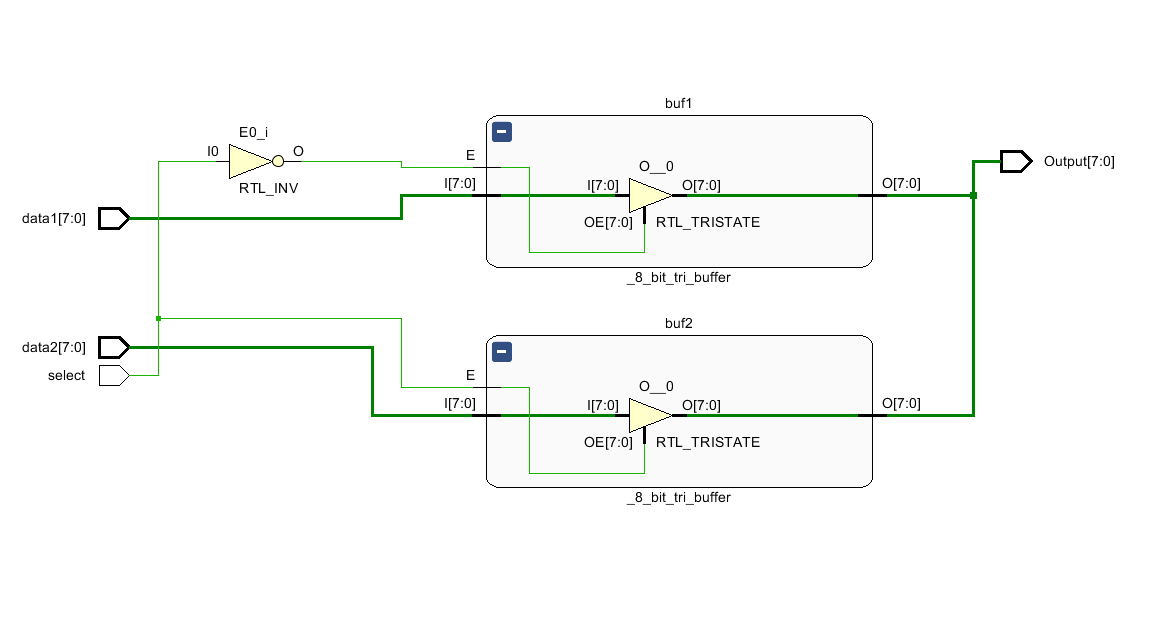
\includegraphics[width=1.0\textwidth]{HW3/Photos/part1_RTL.png}	
	\caption{Design of 8 Bit Bus by Using 3-state Buffers}
	\label{Part 1}
 	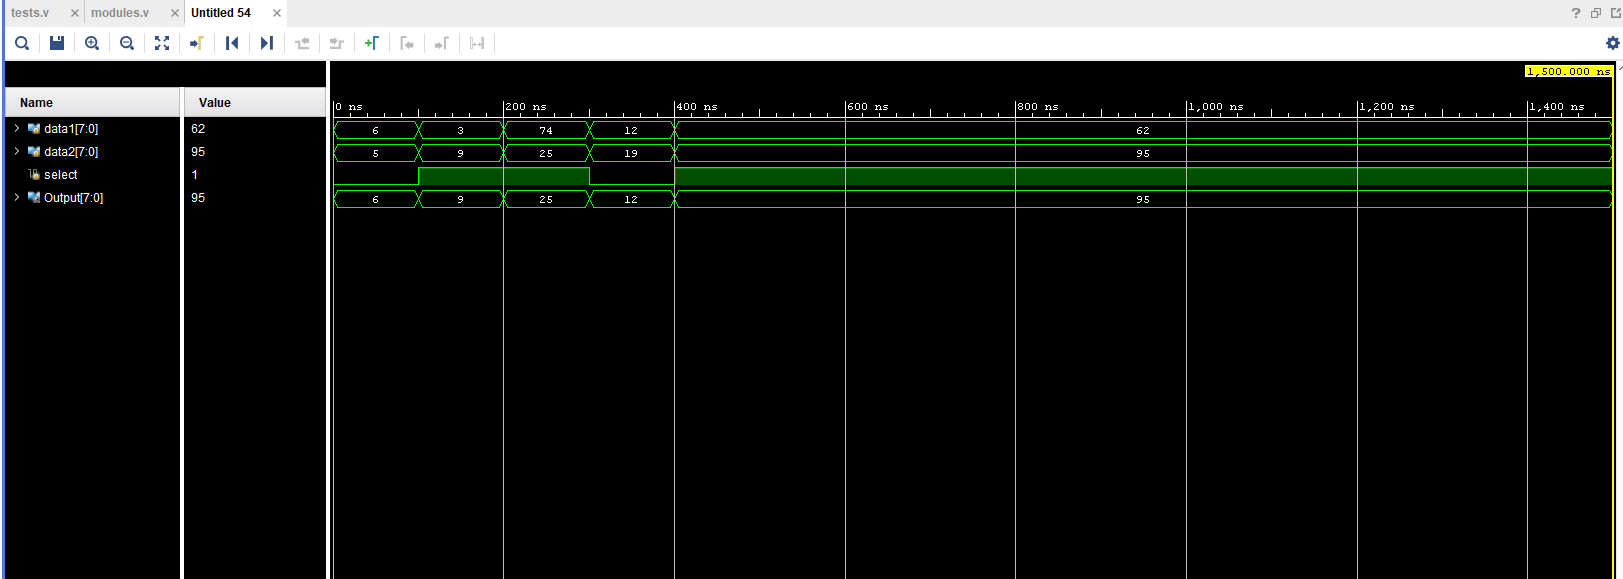
\includegraphics[width=1.0\textwidth]{HW3/Photos/part1_test.png}	
	\caption{Simulation of 8 Bit Bus by Using 3-state Buffers}
	\label{Part 1}
\end{figure}

\subsection{PART 2}
\begin{figure}[ht]
	\centering
	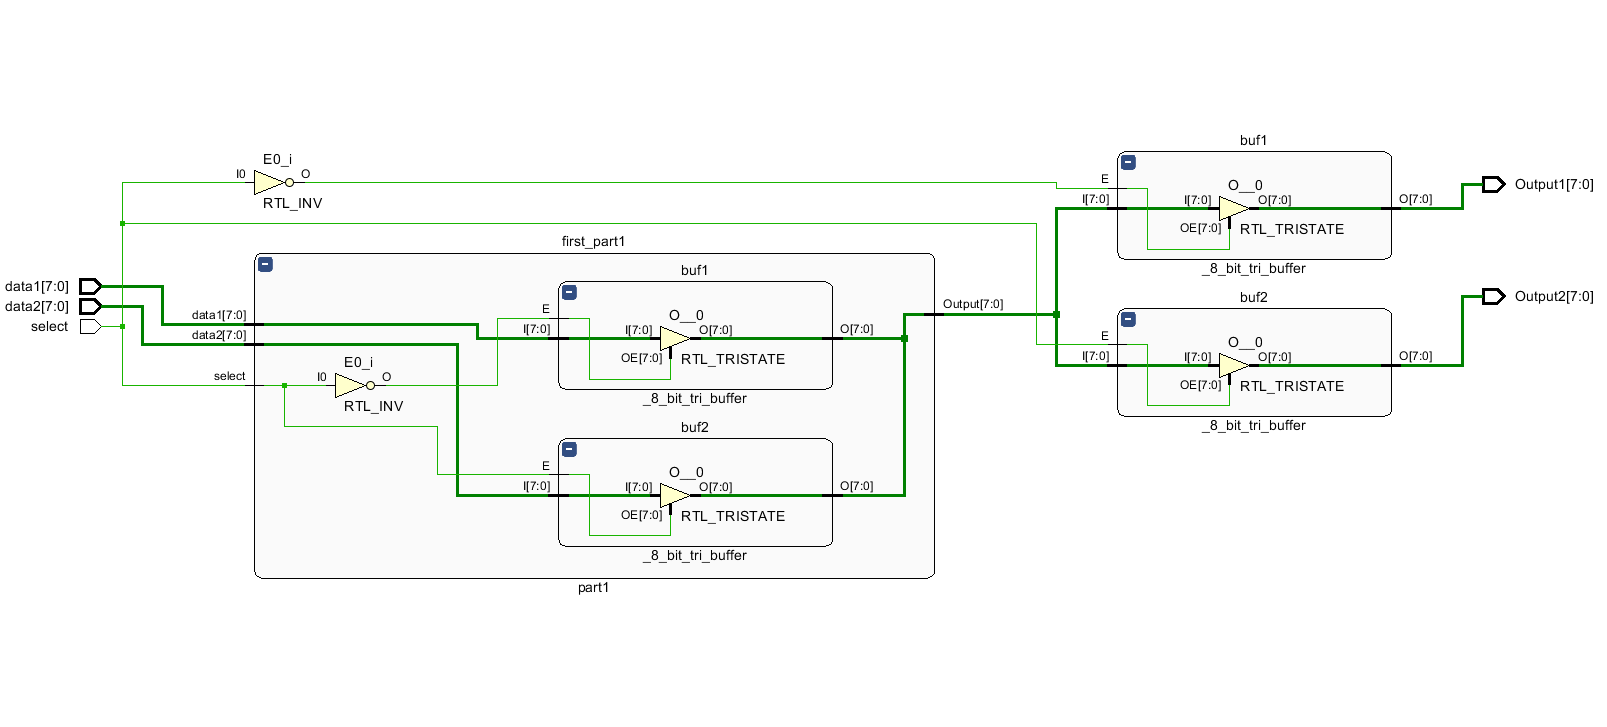
\includegraphics[width=1.0\textwidth]{HW3/Photos/part2_RTL.png}	
	\caption{Design of 8 Bit Data Bus With 2 Drivers and 2 Readers}
	\label{Part 2}
	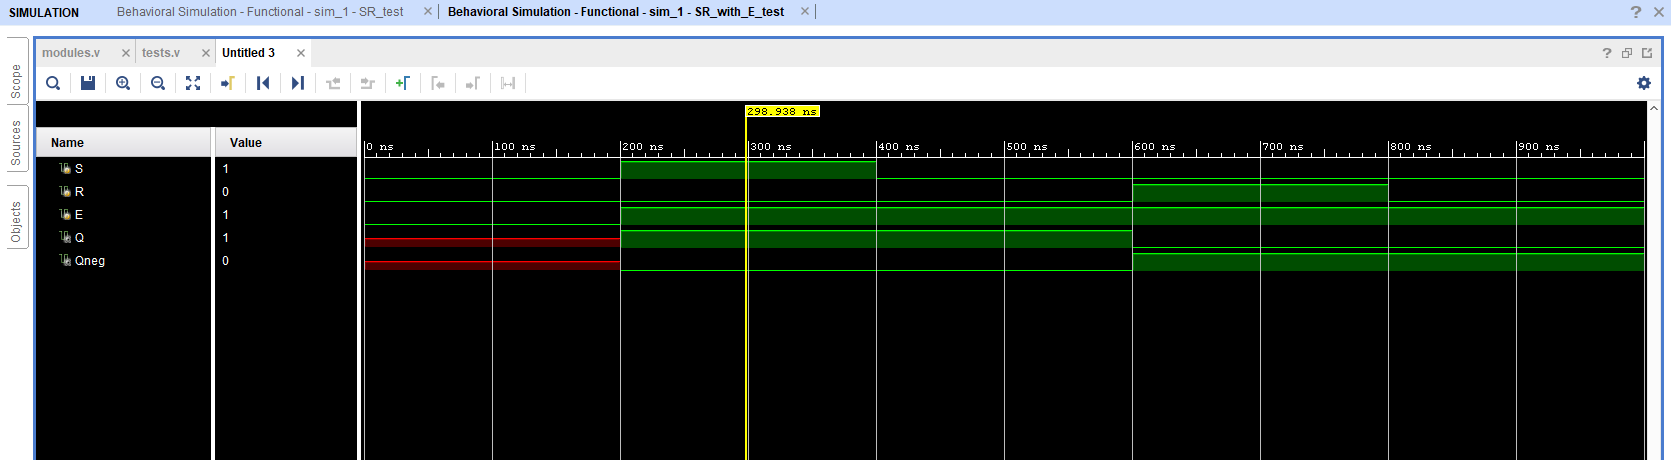
\includegraphics[width=1.0\textwidth]{HW2/Photos/part2_test.png}	
	\caption{Simulation 8 Bit Data Bus With 2 Drivers and 2 Readers}
	\label{Part 2}
\end{figure}

\subsection{PART 3}
\begin{figure}[ht]
	\centering
	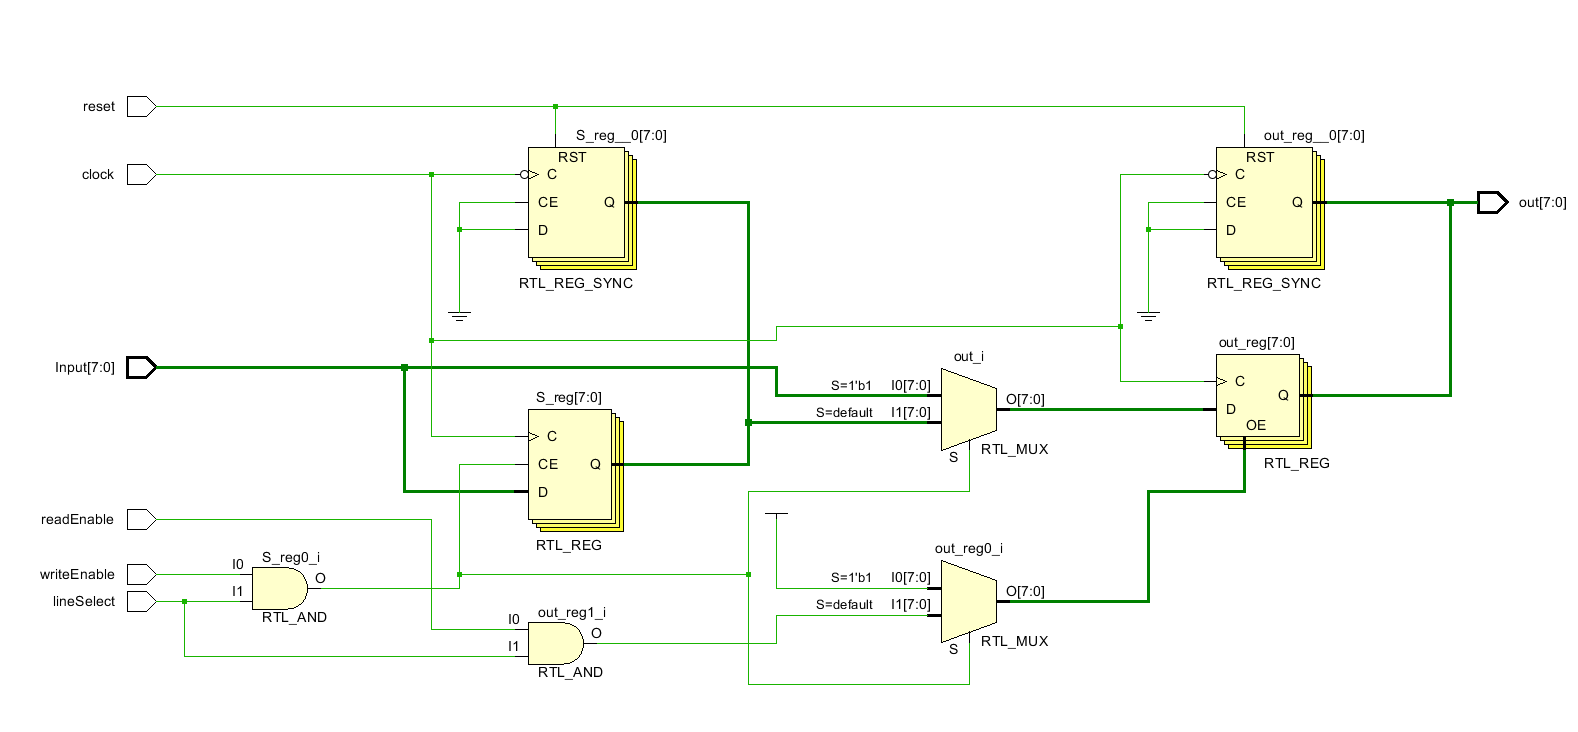
\includegraphics[width=1.0\textwidth]{HW3/Photos/part3_RTL.png}	
	\caption{Design of 8 Bit Memory Line Module}
	\label{Part 3}
        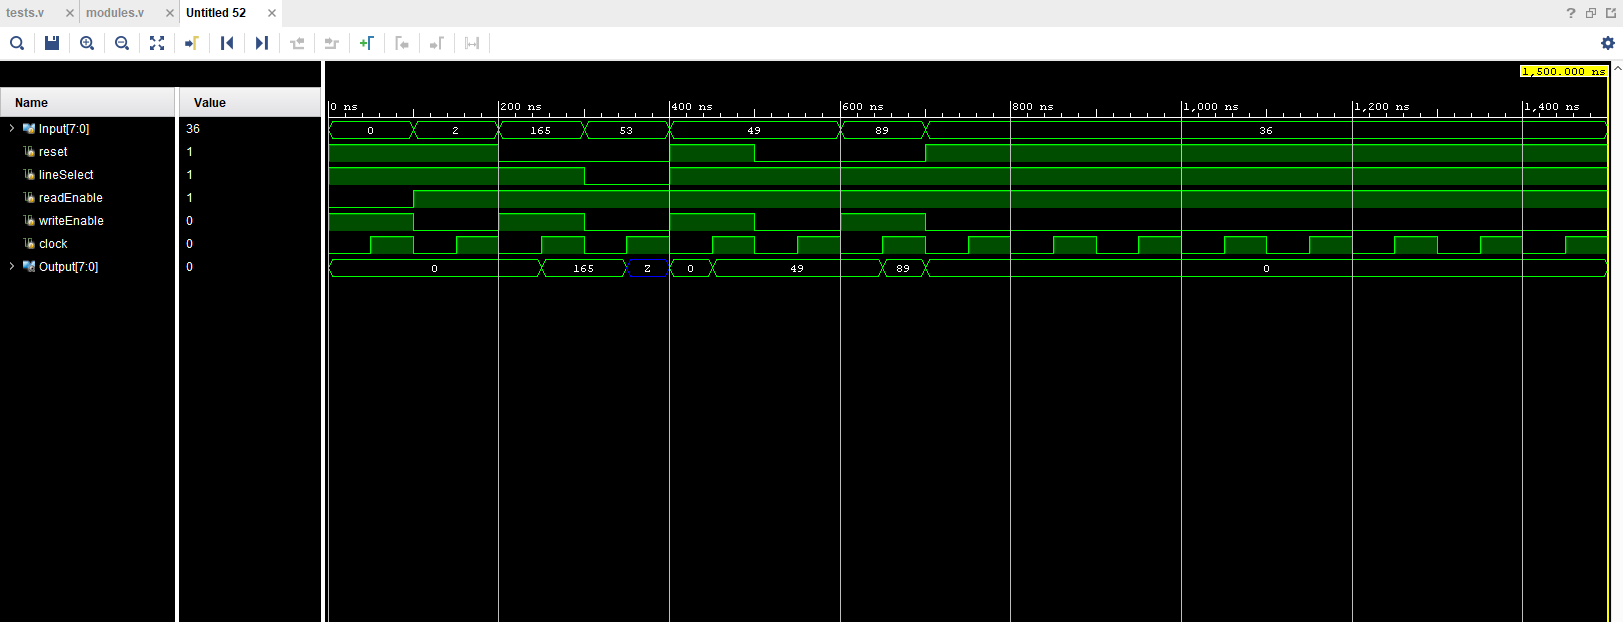
\includegraphics[width=1.0\textwidth]{HW3/Photos/part3_test.png}	
	\caption{Simulation of 8 Bit Memory Line Module}
	\label{Part 3}
\end{figure}

\subsection{PART 4}
\begin{figure}[ht]
	\centering
	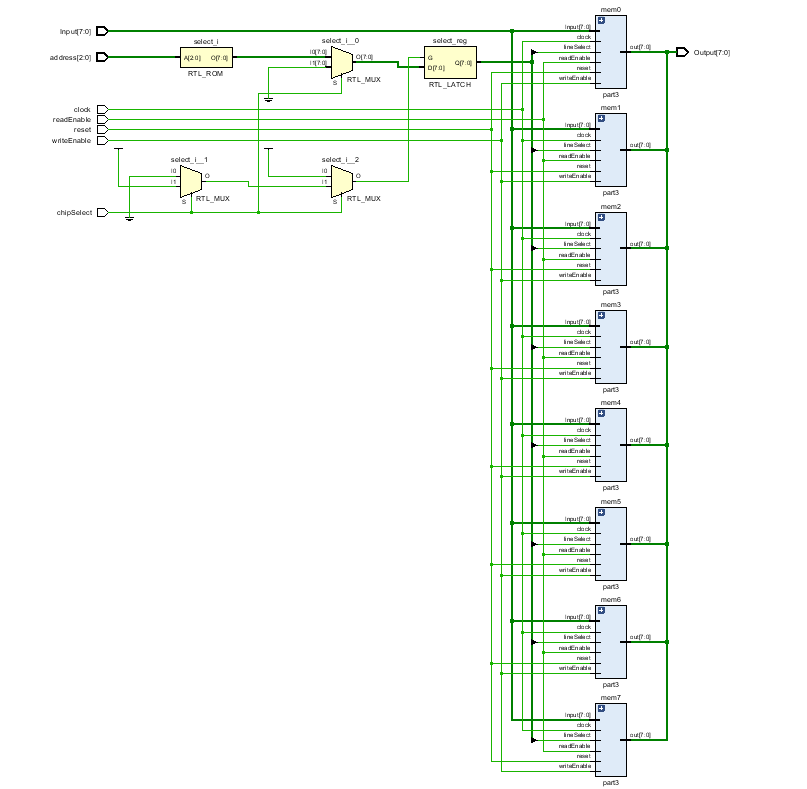
\includegraphics[width=1.0\textwidth]{HW3/Photos/part4_RTL.png}	
	\caption{Design of 8 Byte Memory Module Using 8 Bit Memory Line}
	\label{Part 4}
        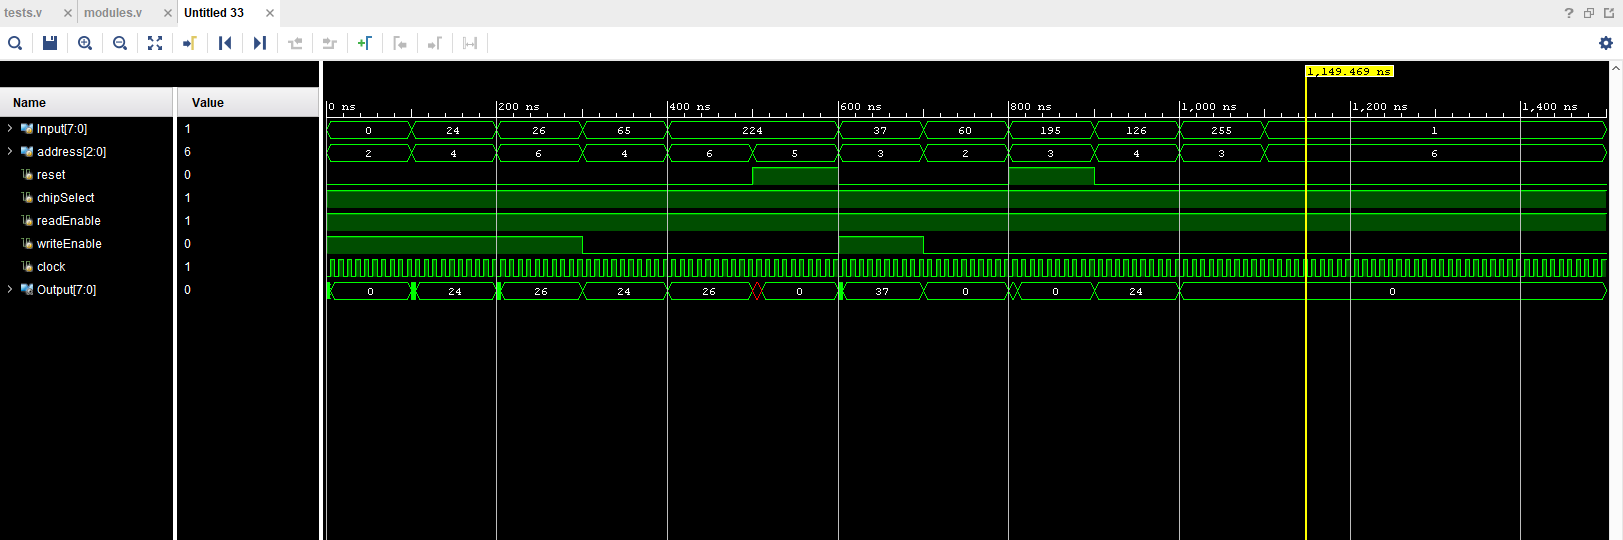
\includegraphics[width=1.0\textwidth]{HW3/Photos/part4_test.png}	
	\caption{Simulation of 8 Byte Memory Module Using 8 Bit Memory Line}
	\label{Part 4}
\end{figure}

\subsection{PART 5}
\begin{figure}[ht]
	\centering
	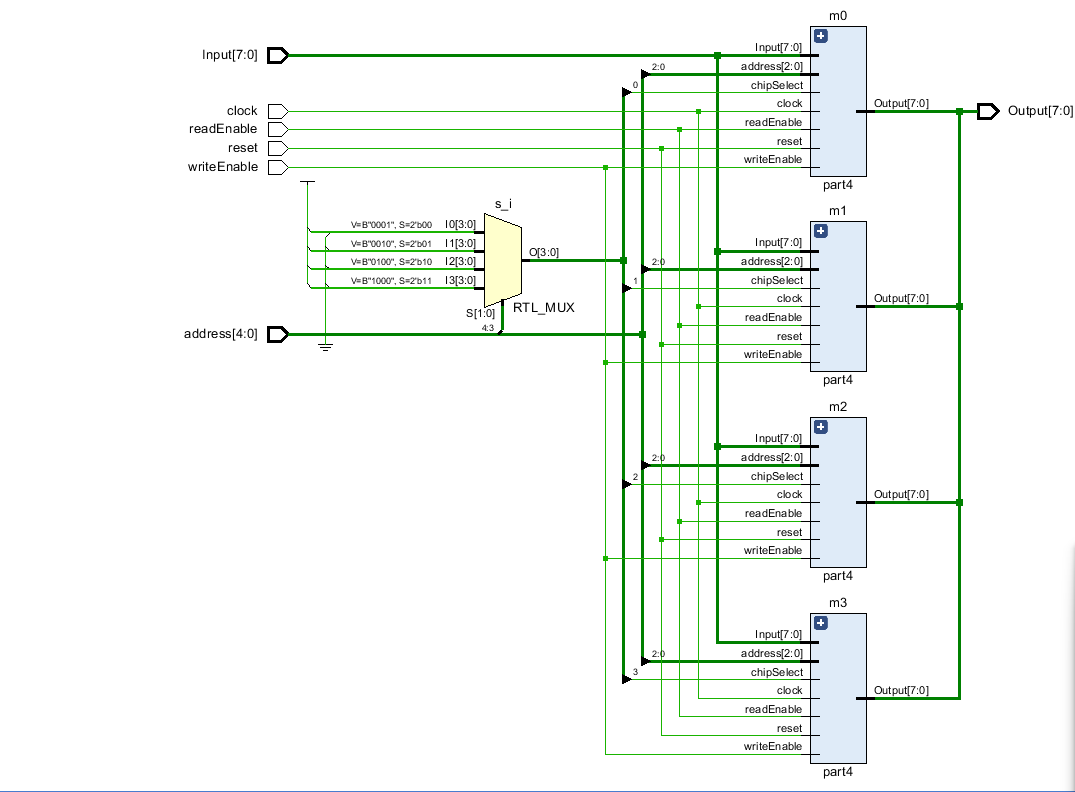
\includegraphics[width=1.0\textwidth]{HW3/Photos/part5_RTL.png}	
	\caption{Design of 32 Byte Memory Module Using 8 Byte Memory}
	\label{Part 5}
        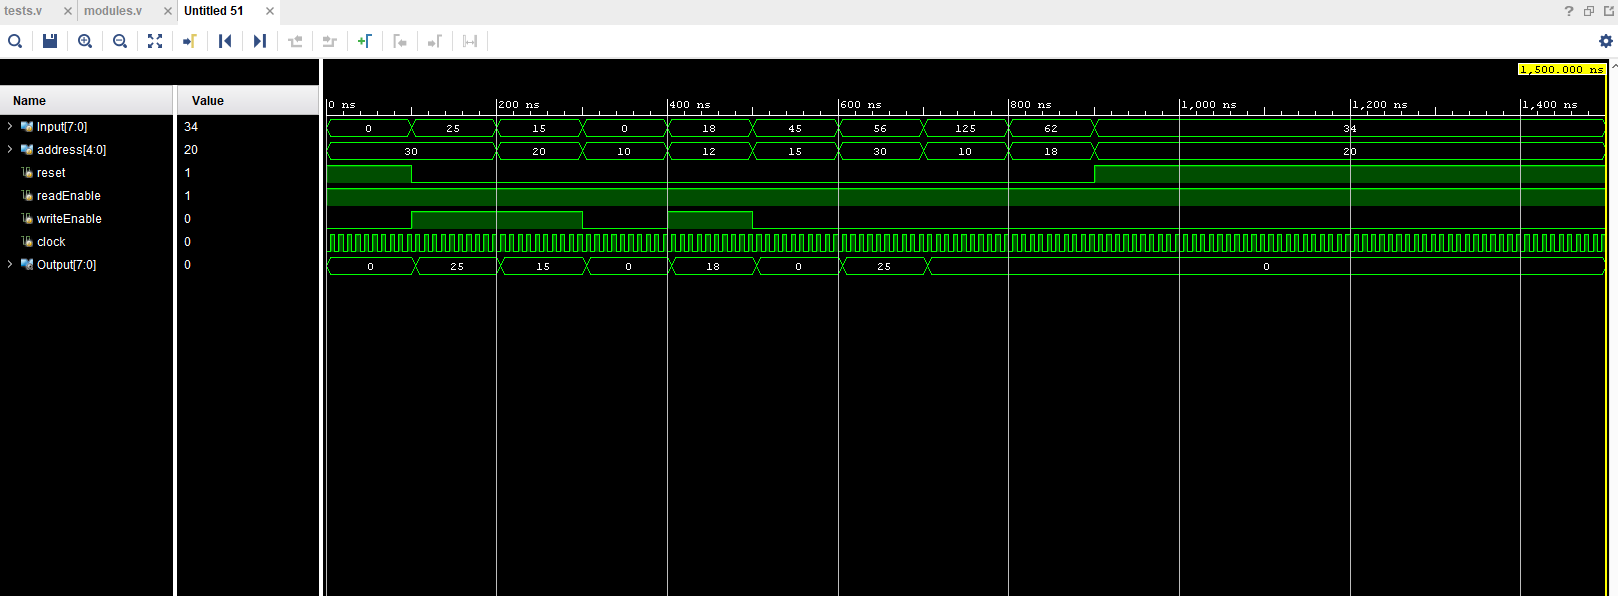
\includegraphics[width=1.0\textwidth]{HW3/Photos/part5_test.png}	
	\caption{Simulation of 32 Byte Memory Module Using 8 Byte Memory}
	\label{Part 5}
 
\end{figure}

\subsection{PART 6}
\begin{figure}[ht]
	\centering
	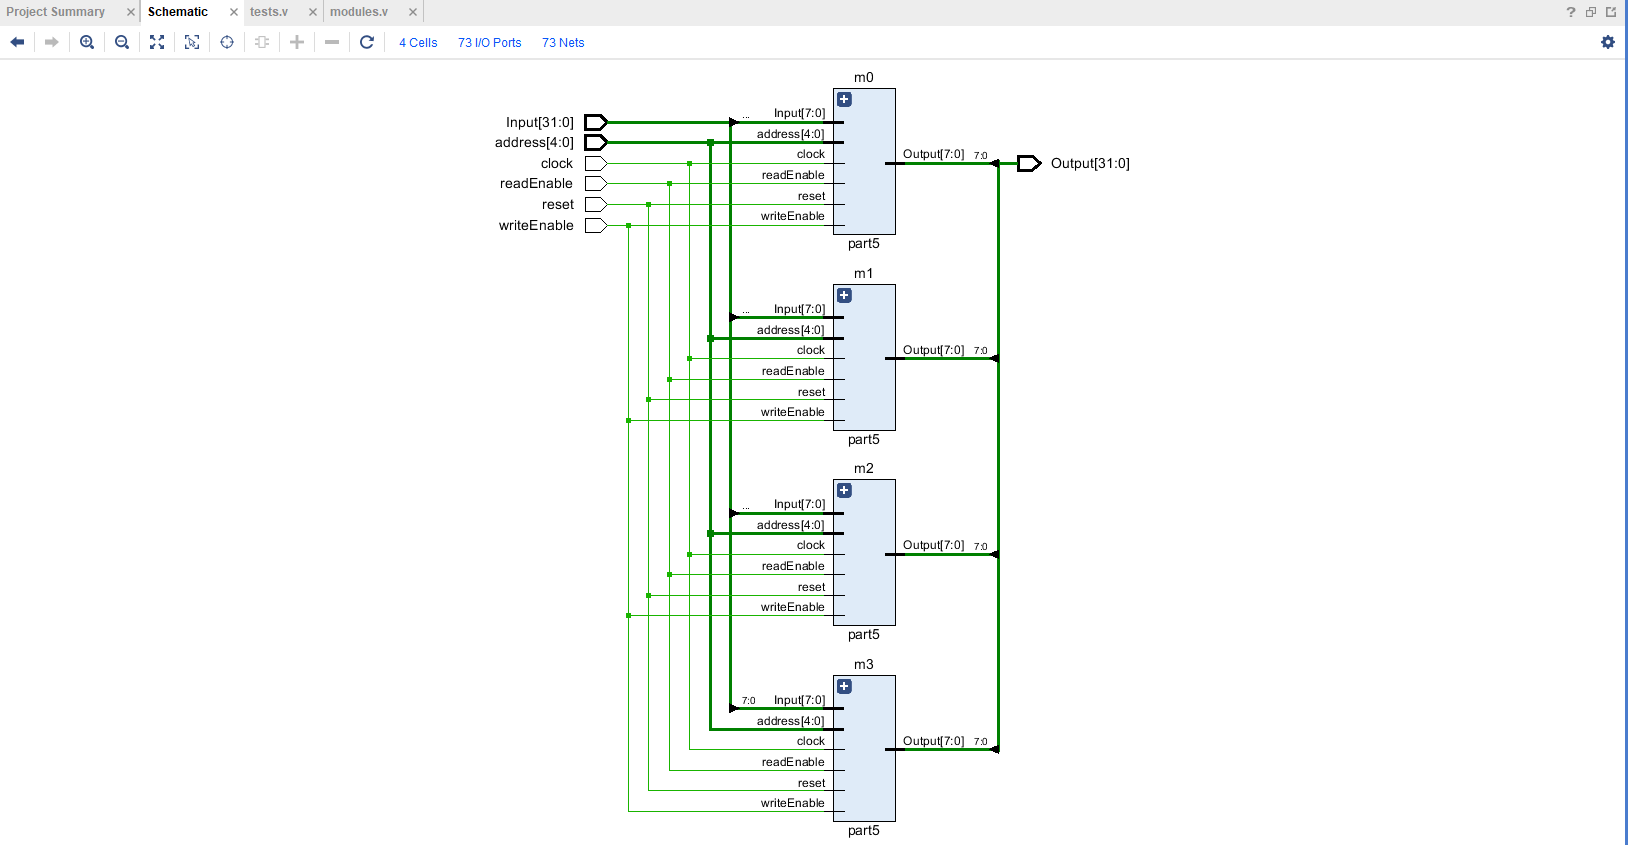
\includegraphics[width=1.0\textwidth]{HW3/Photos/part6_RTL.png}	
	\caption{Design of 128 Byte Memory Module With 32 Byte Memory}
	\label{Part 6}
 	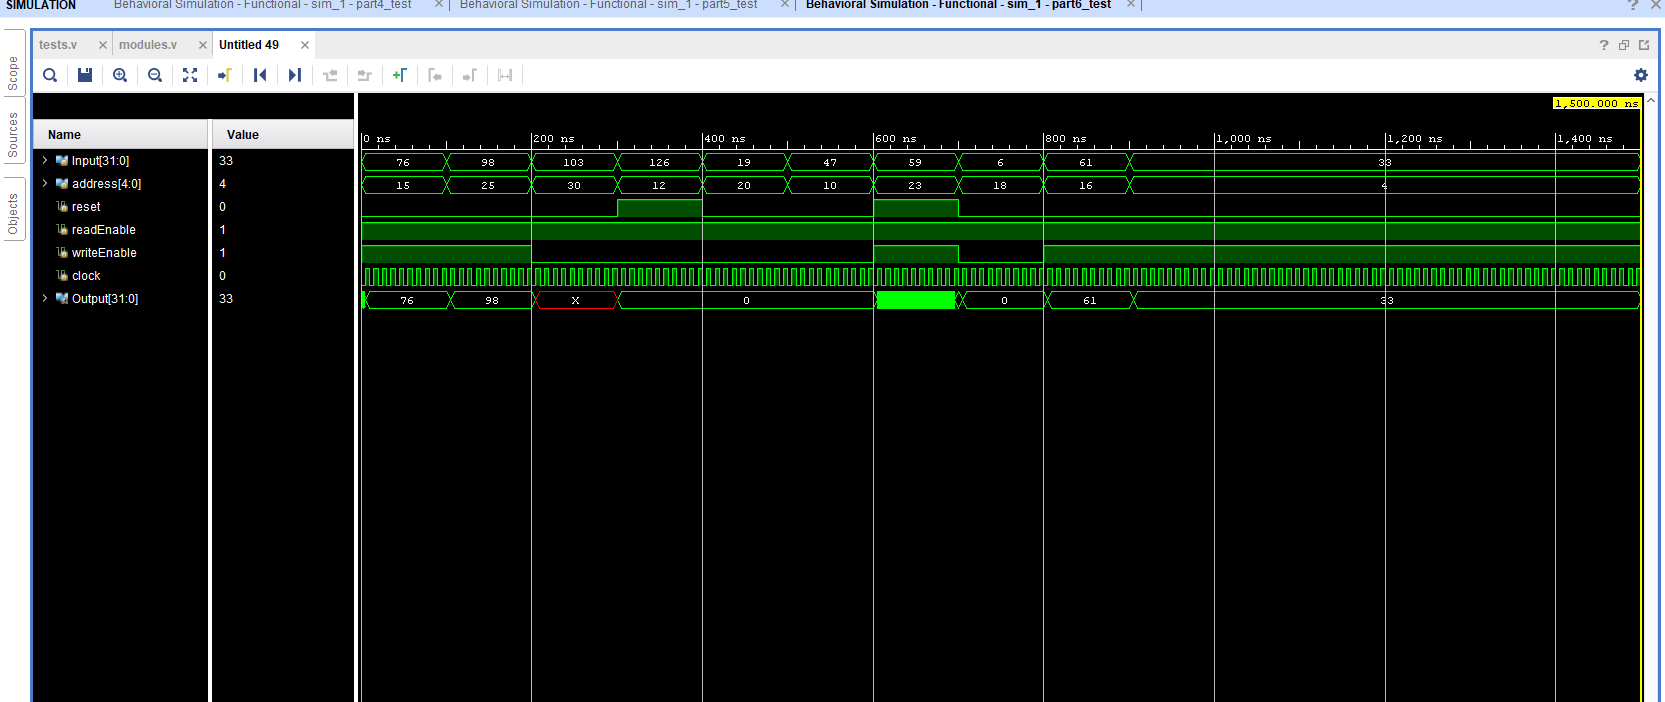
\includegraphics[width=1.0\textwidth]{HW3/Photos/part6_test.png}	
	\caption{Simulation of 128 Byte Memory Module With 32 Byte Memory}
	\label{Part 6}
\end{figure}



\section{RESULTS}
Using Verilog, various memory types has been built. Usage of bus has been indicated with this implementation.

\section{DISCUSSION}
 Different memories has been implemented such as 8 bit, 8 byte, 32 byte, and 128 byte. We have used smaller memory types to build bigger ones. Also we have used a bus with three-state buffers which we have already implemented in first two parts while we implementing memories.

\section{CONCLUSION}
We have recalled the design of three-state buffer and used for implementing a bus system. We have learned implementing memory with Verilog and examined read, write and reset operations with simulation sources.

\newpage
\addcontentsline{toc}{section}{\numberline {}REFERENCES}

\bibliographystyle{unsrt}
\bibliography{reference}

\end{document}

